\section{Cylc Overview}
\label{Cylc Overview}

\note{For more information on the topics of this section, see Appendix~\ref{Appendix
Cylc Overview} and the Cylc User Guide.}

Cylc (``silk'') is a workflow engine that can manage continuous workflows of
cycling (repeating) tasks for applications such as weather and environmental
forecasting, and climate simulation.

\begin{itemize}
    \item \terminology{A \underline{task} represents a \underline{job} (a script or
program) that runs on a computer.}
    \item \terminology{A \underline{workflow} is a \underline{suite} of interdependent
tasks.}
    \item \terminology{A \underline{cycle point} is a point on an integer or
        date-time sequence.}
    \item \terminology{A \underline{cycling task} runs the same job repeatedly for some
sequence of cycle points.}
    \item \terminology{A \underline{continuous workflow of cycling tasks} is a single
workflow, not just a sequence of single-cycle workflows, and it may extend
indefinitely into the future.} 
\end{itemize}

A small workflow of six tasks (with no cycling as yet) can be shown as a {\em
dependency graph}:

\begin{center}
    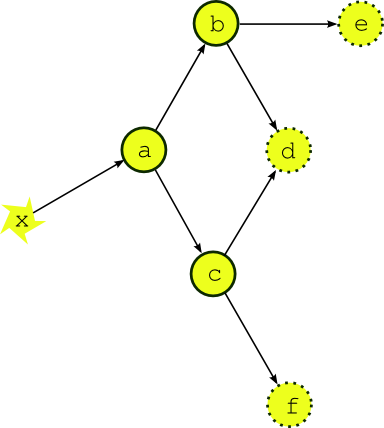
\includegraphics[width=0.25\columnwidth]{resources/tex/dep-one-cycle}
\end{center}

where the graph {\em nodes} represent tasks, and {\em edges} (arrows) represent
dependence.  Task {\em a} might write out data files that are read in by tasks
{\em b} and {\em c}, for instance.  The node {\em x} here represents an
external event such as receipt of new real-time data (weather observations,
perhaps).

Before cycling this workflow  we should be aware of {\em inter-cycle
dependence}.  For example, task {\em a} may depend on restart files generated
by its own previous instance, like this:

\begin{center}
    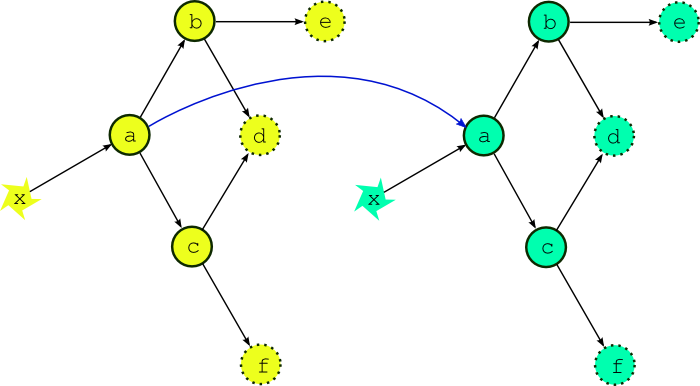
\includegraphics[width=0.5\columnwidth]{resources/tex/dep-two-cycles-linked}
\end{center}

This inter-cycle dependence can be ignored {\em if} we agree always to finish
one complete cycle before starting the next.  This is usually the case in
operational systems where there's a wait between cycles for new real time data
(such as the latest weather observations).  But if the suite has to catch up
from a delay, or if we run it over archived historical data, we should be able
to run tasks from multiple cycles at once for more efficient scheduling.  Here,
according to the dependencies shown, if green {\em x} is already done then
green {\em a} should be able to start at the same time as yellow {\em b}
and {\em c}, as soon as yellow {\em a} is finished.

Traditional fixed-cycling schedulers can't do this because they ignore
inter-cycle dependence and must therefore run complete cycles
sequentially.\footnote{Although some mitigate this problem by statically
defining multiple steps or ``chunks'' within fixed cycles.}

Cylc knows about inter-cycle dependence and manages the suite as {\em a single
continuous workflow with no cycle boundaries}, not as a series of distinct
single-cycle-point workflows.  In cylc, cycle points are merely task labels,
not global loop indices.  Each task can run when its own inputs are satisfied,
regardless of cycle point.  Here's how cylc sees three cycles of our example
suite (note that this can go on indefinitely):

\begin{center}
    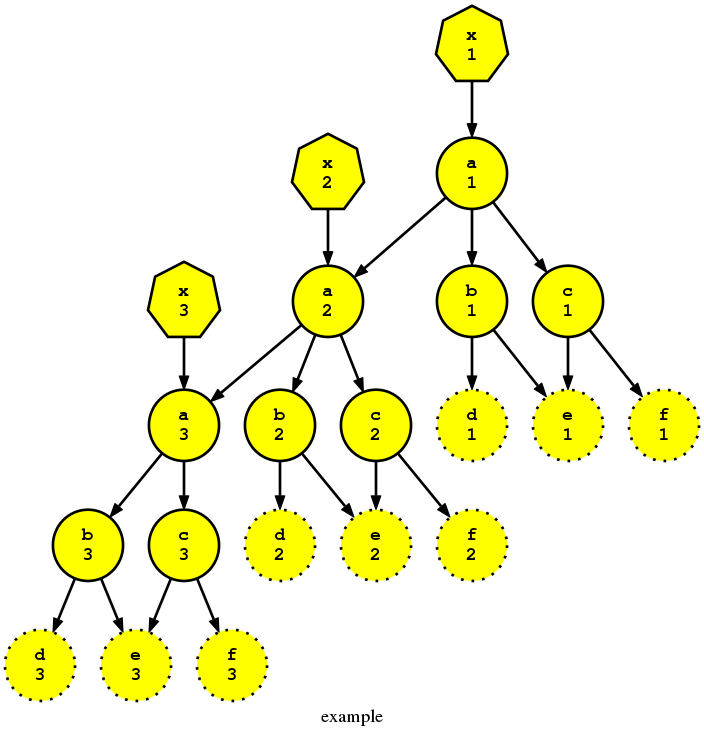
\includegraphics[width=0.45\columnwidth]{resources/example-3cycles.png}
\end{center}

Consequently, cylc can run workflows faster, recover from delays faster, and
handle failures and delays better than fixed-cycle schedulers.
Appendix~\ref{Appendix Cylc Overview} shows actual job schedules for this
example suite, and compares the result for a fixed-cycle scheduler.
